\documentclass{amsart}
\usepackage[margin=3cm]{geometry}                % See geometry.pdf to learn the layout options. There are lots.
\geometry{letterpaper}                   % ... or a4paper or a5paper or ...
%\geometry{landscape}                % Activate for for rotated page geometry
\usepackage[parfill]{parskip}    % Activate to begin paragraphs with an empty line rather than an indent
\usepackage{float}
\usepackage{graphicx}
\usepackage{amssymb}
\usepackage{epstopdf}
\usepackage{siunitx}
\usepackage{subcaption}
\usepackage{units}
\usepackage{setspace}

\DeclareGraphicsRule{.tif}{png}{.png}{`convert #1 `dirname #1`/`basename #1 .tif`.png}
\graphicspath{{./img/}}


\title{      }
\author{Caspar \textsc{Lant}} % Author name

\date{\today} % Date for the report

\begin{document}

\bigskip

\maketitle % Insert the title, author and date
\begin{center}

Intermediate Experimental Physics II\\
\vspace{1.5cm}

\begin{tabular}{l r}

Section: & 001\\
\\
Date Performed: & March 15, 2016 \\ % Date the experiment was performed
Date Due: & March 22, 2016\\
\\
Partner: & Neil Saddler\\ % Partner names
Professor: & Prof. Andrew Kent\\
Instructor: & David Mykytyn % Instructor/supervisor
\end{tabular}
\vfill
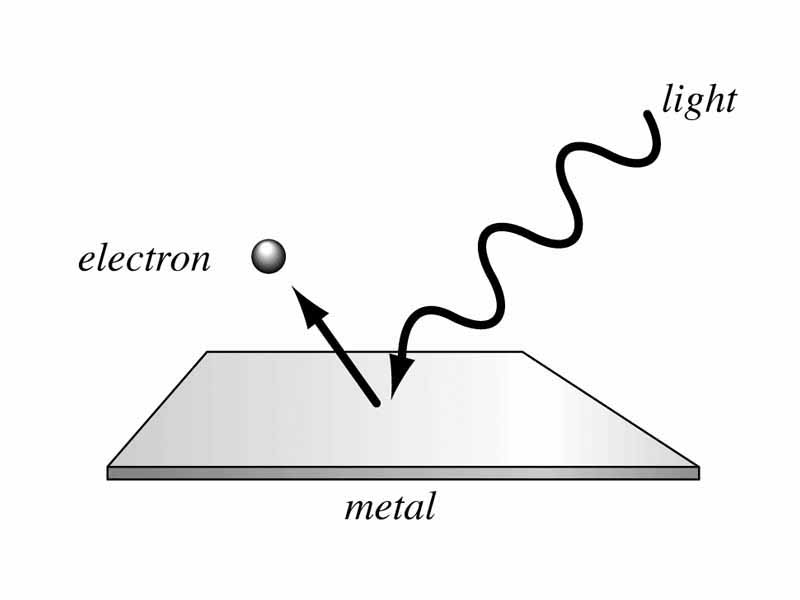
\includegraphics[width=.7\textwidth]{diagram.jpg}
\end{center}
\vfill
\pagebreak

\setstretch{1.5}
\paragraph{\textbf{The Objective} of this week's experiment was to put our vast theoretical knowledge of lenses to application. It is always a remarkable think to see what was once pure abstraction validated though rigorous scientific experimentation. }

\section{Theoretical Background/ Abstract}
\paragraph{Electrons are held inside metals by electric forces. For a given metal at room temperature, where thermal effects are negligible, an electron must be given a minimum amount of energy to escape from the metal. This minimum amount of energy is called the work function φ. Energy can be supplied to the electrons by shining light onto the metal surface. Electrons that have been liberated from the metal by this mechanism are called photoelectrons. If monochromatic light is incident on a metal surface it is found that if the frequency of the light is less than a given frequency, called the threshold frequency ν0, no electrons are emitted however intense the light and no matter how long you wait. If the frequency of the light is above the threshold frequency, electrons are emitted almost immediately even if the light intensity is very small. These facts cannot be explained on a classical basis in which the light is considered to be oscillating electric and magnetic fields. In 1905 Albert Einstein explained this mystery by assuming that the energy of light was not continuous but discrete. The light energy was quantized in massless particles called photons each with energy hν. Planck’s constant is h and ν is the frequency of the light. An electron absorbs the entire energy of a photon or absorbs no energy at all. This simple explanation was worth a Nobel prize. Light has the usual wave-particle duality of matter. For some problems it is necessary to treat light as a wave and for other problems as a particle.\\
Photoelectrons arise from the electrons in the conduction band of a metal. A very simple model, illustrated in Fig. 1, gives the salient features. The electrons are held inside the metal by a potential energy step. The potential energy is constant on either side of the step, and we take the potential energy as zero inside the metal. Inside the metal the electrons fill up all the available energy states up to maximum energy Emax. There are almost no electrons with energy greater than Emax, assuming the temperature is low. The energy from Emax to the top of the potential energy step is the work function φ = hν0. When an electron inside the metal of a given energy approaches the surface, a force is exerted on it that reflects the electron from the surface. Consider an electron inside the metal with energy Emax. If this electron absorbs a photon of energy hν, The maximum kinetic energy Kmax that this
electron can have if it leaves the metal is}
\begin{equation}
    K_{max} = h\nu - \phi
\end{equation}
\begin{equation}
    V_s = \dfrac{h}{\rm e} \nu - \dfrac{\phi}{\rm e}
\end{equation}

\section{Experimental Procedure}
\begin{enumerate}
    \item Plug everything in in the manner depicted in the schematic.
    \item Now that I know that you don't read the procedure section, typing them up has become so much more laborious.
    \item
    \item
    \item
    \item
    \item
    \item
    \item
    \item
    \item
    \item
    \item
    \item
\end{enumerate}

\section{Graphs and Tables}

\begin{table}[H]
    \begin{minipage}{.45\textwidth}
\centering
\caption{Voltage vs. Deflection}
\bigskip \bigskip
\label{my-label}
\begin{tabular}{c|c|c|c}
Voltage (V) & 546nm & 577nm & 435nm \\ \hline
0.0         & 22.0  & 4.9   & 60.5  \\
0.1         & 16.0  & 3.3   & 47.8  \\
0.2         & 10.1  & 2.0   & 33.9  \\
0.3         & 5.0   & 0.9   & 21.5  \\
0.4         & 1.7   & 0.1   & 11.7  \\
0.5         & -0.1  & 0.0   & 4.0   \\
0.6         & -0.9  & 0.0   & -1.2  \\
0.7         & -1.2  & 0.0   & -5.0  \\
0.8         & -1.3  & 0.0   & -7.5  \\
0.9         & -1.4  & 0.0   & -9.0  \\
1.0         & -1.4  & 0.0   & -10.0 \\
1.1         & -1.5  & 0.0   & -10.5 \\
1.2         & -1.5  & 0.0   & -10.9 \\
1.3         & -1.5  & 0.0   & -11.0 \\
1.4         & -1.5  & 0.0   & -11.1 \\
1.5         & -1.5  & 0.0   & -11.1 \\
1.6         & -1.5  & 0.0   & -11.1 \\
1.7         & -1.5  & 0.0   & -11.1 \\
1.8         & -1.5  & 0.0   & -11.1 \\
1.9         & -1.5  & 0.0   & -11.1 \\
2.0         & -1.5  & 0.0   & -11.1 \\
2.1         & -1.5  & 0.0   & -11.2 \\
2.2         & -1.5  & 0.0   & -11.2 \\
2.3         & -1.5  & 0.0   & -11.2 \\
2.4         & -1.5  & 0.0   & -11.2 \\
2.5         & -1.5  & 0.0   & -11.3 \\
2.6         & -1.5  & 0.0   & -11.3 \\
2.7         & -1.5  & 0.0   & -11.3 \\
2.8         & -1.5  & 0.0   & -11.3 \\
2.9         & -1.5  & 0.0   & -11.4
\end{tabular}
\end{minipage}
%
\begin{minipage}{.5\textwidth}
    \centering
    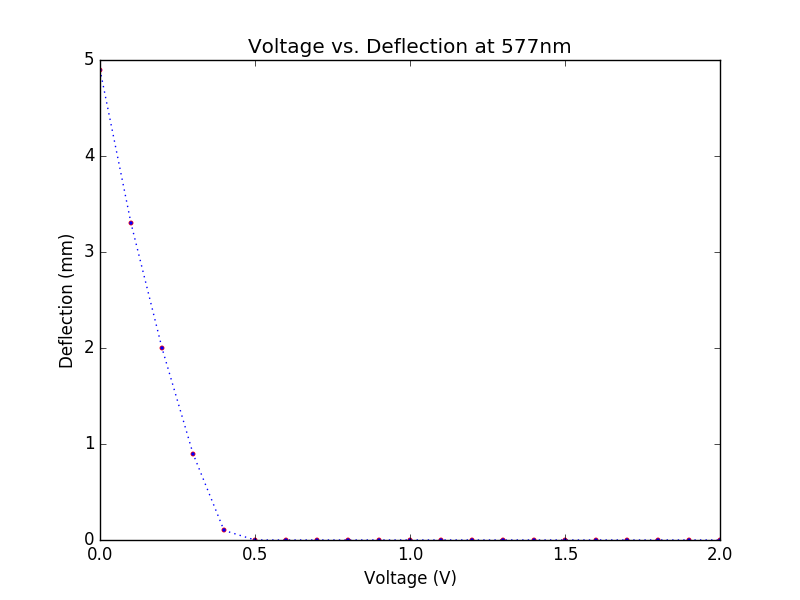
\includegraphics[height=.23\textheight]{577.png}\\
    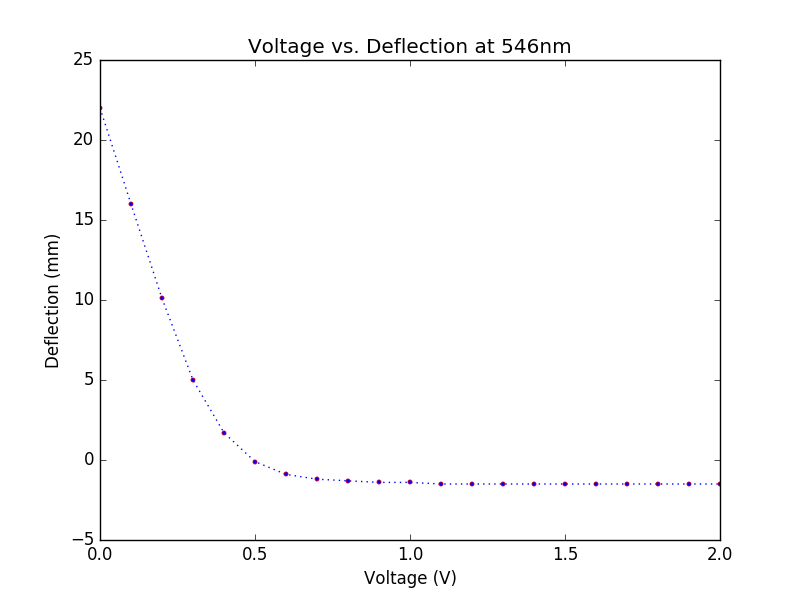
\includegraphics[height=.23\textheight]{546.png}\\
    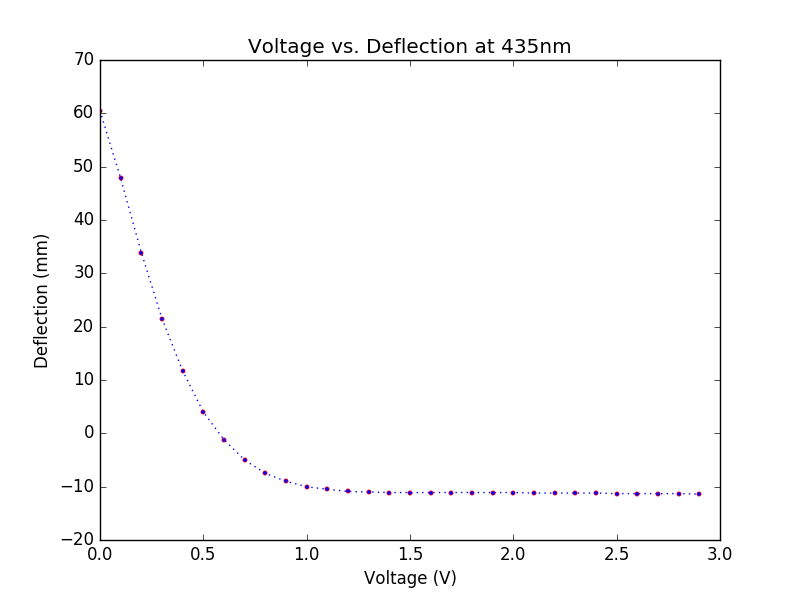
\includegraphics[height=.23\textheight]{435.png}
\end{minipage}
\end{table}

\begin{figure}
    \begin{minipage}{.45\textwidth}
        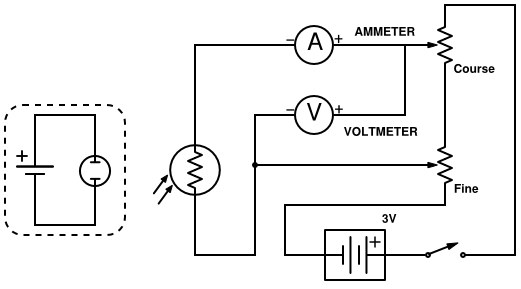
\includegraphics[width=\textwidth]{schematic.png}
    \end{minipage}
    %
    \begin{minipage}{.45\textwidth}

    \end{minipage}
\end{figure}

The topmost plot corresponds to a filter of slit width 577 nm, the middle plot 546 nm, and the last plot a wavelength of 435 nm.
\section{Questions}

\begin{enumerate}
    \item {\textit{Question?}
\begin{quote}
Answer
\end{quote}}

\item{\textit{Question?}
\begin{quote}
Answer
\end{quote}}

\end{enumerate}

\section{Error Analysis}




\end{document}
